\section{A shared activity}

Everyone can do it, including the robot.
Active segmentation.


A robot equipped with an arm and an active vision head was given a
simple
``poking'' behavior, whereby it selected objects in its environment,
and tapped them lightly while fixating them~\citep{fitzpatrick02towards}.
%
The motion signature generated by the impact of the arm with a rigid
object greatly simplifies segmenting that object from its background,
and obtaining a reasonable estimate of its
boundary (see Figure~\ref{fig:separate-simple}).

PENDING: preemption as a good way of giving human demos.



Get lots of object segmentations, tracked motion.  
Cluster them.  Now can differentiate between objects,
can see how they respond to poking individually.
%
At this point can support basic mimicry (figures?).



\begin{figure}[bt]
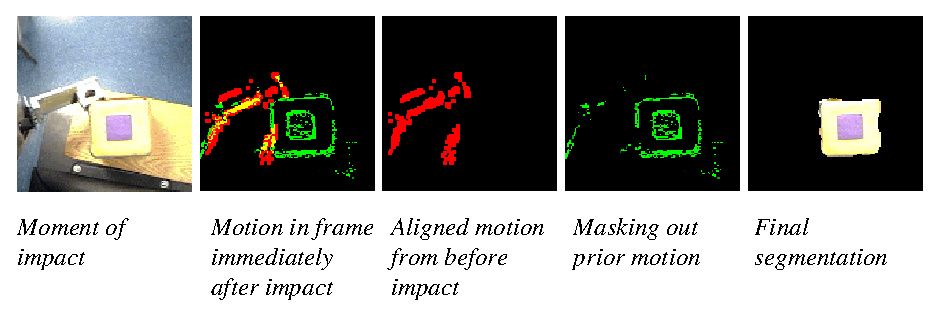
\includegraphics[width=\columnwidth]{fig-separate-simple}
\caption
{
\label{fig:separate-simple}
%
Active segmentation.  The robot arm is deliberately driven
to collide with an object.
 The
apparent motion after contact, when masked by the motion before
contact, identifies a seed foreground (object) region.  Such motion
will generally contain fragments of the arm and environmental motion
that escaped masking.  Motion present before contact is used to
identify background (non-object) regions.  
An optimal object region is computed from the foreground and
background information using graph cuts~\citep{fitzpatrick03first}.
%
%This prevents the region
%assigned to the object motion from growing to include these fragments.
%The largest connected region, with a minor post-processing clean-up,
%is taken as the official segmentation of the object.
%
}
\end{figure}



Active segmentation was recruited as a developmentally plausible means
of initiating early integration of vision and manipulation as part of
a large-scale experiment aimed at implementing a robotic analogue of
the mirror-neuron system found in primates~\cite{self02omit}.  The
robot was given a poking behavior so that it would extend its arm to
swing near anything reachable that its attention system was directed
towards.  A human caregiver brought interesting objects to the robot
to poke.  The objects differed in how they rolled, and the robot
learned to exploit that fact.  Active segmentation played two roles in
this experiment: collecting data for later object recognition and
localization, and providing a good segmentation for tracking the
motion of the object after contact.  End to end performance of the
system was described in~\cite{self02omit}.  Here we report on the
performance of the active segmentation component in isolation.
